\nxsection{Le r\^ole ''Manager''}\label{sec:utilisateurs-vendeur}
\index{vendeur}
\index{Vendeur}

La figure~\ref{fig:yeren-fenetre-patron} illustre la fen\^etre
d'acceuil d'un utilisateur avec le \role \manager, 
apr\`es qu'il se soit enregistr\'e dans \yeren.\\

\begin{figure}[!htbp]
\centering
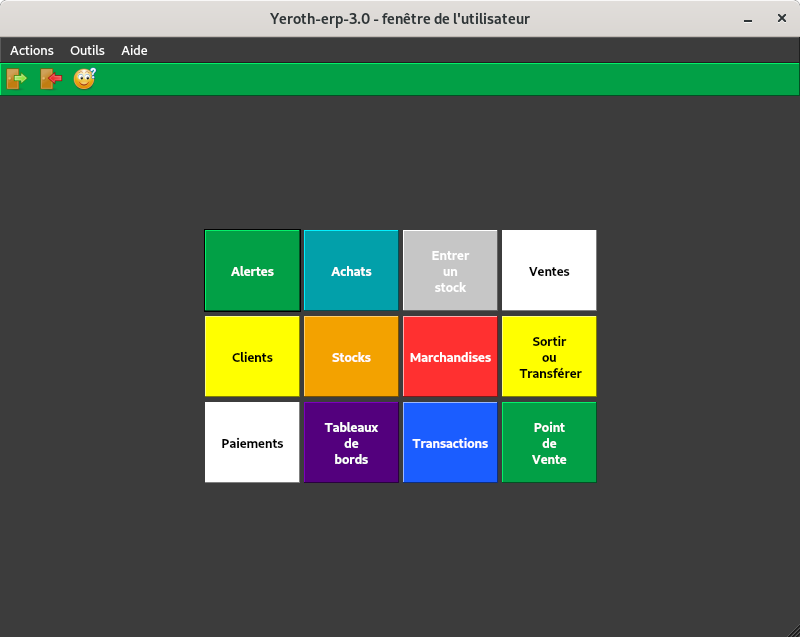
\includegraphics[scale=0.63]{images/yeroth-fenetre-manager.png}
\caption{La fen\^etre d'acceuil d'un ''manager''}
\label{fig:yeren-fenetre-patron}
\end{figure}

Un utilisateur de \yeren avec le \role "\manager" a
acc\`es \`a toutes les fonctionalit\'es de \yeren. Il
cumule les t\^aches de d'administrateur, de magasinier,
et de caissier.

Le \role \manager est le seul \`a donner acc\`es aux
informations des ventes dans leurs totalit\'es, ainsi
qu'\`a la g\'en\'eration et \`a la consultation des
rapports commerciaux.

Le \role \manager est le seul \`a pouvoir consulter toutes
les alertes re\c{c}ues par les autres utilisateurs, et
\`a pouvoir les supprimer.